
%(BEGIN_QUESTION)
% Copyright 2006, Tony R. Kuphaldt, released under the Creative Commons Attribution License (v 1.0)
% This means you may do almost anything with this work of mine, so long as you give me proper credit

A form of liquid level switch called a {\it tilt switch} is often used for detecting sewage level in ``lift stations'' where sewage collected from homes via gravity is pumped out of the collection sump to the wastewater treatment plant (usually located miles away):

$$\includegraphics[width=15.5cm]{i00303x01.eps}$$

Tilt switches often use a small glass vial containing liquid mercury as the tilt sensor.  Explain how a glass tube partially filled with mercury works as an electrical tilt switch, and also perform a ``thought experiment'' where you describe this system's function from start to finish through a complete start-stop cycle of the pump motor:

$$\includegraphics[width=15.5cm]{i00303x02.eps}$$

\vskip 20pt \vbox{\hrule \hbox{\strut \vrule{} {\bf Suggestions for Socratic discussion} \vrule} \hrule}

\begin{itemize}
\item{} What would happen if the OL switch failed open in this system?
\item{} What would happen if the LSL switch failed open in this system?
\item{} What would happen if the LSH switch failed open in this system?
\item{} What would happen if the LSL switch failed shorted in this system?
\item{} What would happen if the LSH switch failed shorted in this system?
\item{} What would happen if the LSH switch failed shorted in this system?
\item{} What would happen if the M1 seal-in contact failed open in this system?
\item{} What would happen if the M1 seal-in contact failed shorted in this system?
\end{itemize}

\underbar{file i00303}
%(END_QUESTION)





%(BEGIN_ANSWER)

Be sure to review the operation of this simple motor start-stop circuit in your answer!

%(END_ANSWER)





%(BEGIN_NOTES)

A mercury ``tilt switch'' uses a sample of liquid mercury metal to bridge wire contacts inside of a sealed glass tube when the tube is tipped in a certain direction.

\vskip 10pt

\noindent
Thought experiment:

\begin{itemize}
\item{} Sump starts empty
\item{} Level begins to rise
\item{} LSL switch tilts; motor doesn't start up yet because LSH is still open
\item{} LSH switch tilts; motor starts up
\item{} Level begins to drop as pump moves wastewater out of sump
\item{} LSH returns to normal; motor continues to run because it's control circuit is ``sealed in''
\item{} LSL retuns to normal; motor stops and remains off until LSH tips again
\end{itemize}










\filbreak \vskip 20pt \vbox{\hrule \hbox{\strut \vrule{} {\bf Virtual Troubleshooting} \vrule} \hrule}

\noindent
{\bf Predicting the effect of a given fault:} present each of the following faults to the students, one at a time, having them comment on all the effects each fault would produce.

\begin{itemize}
\item{} 
\item{} 
\item{} 
\end{itemize}


\vskip 10pt


\noindent
{\bf Identifying possible/impossible faults:} present symptoms to the students and then have them determine whether or not a series of suggested faults could account for all the symptoms, explaining {\it why} or {\it why not} for each proposed fault:

\begin{itemize}
\item{} Symptom: {\it }
\item{}  -- {\bf Yes/No}
\item{}  -- {\bf Yes/No}
\item{}  -- {\bf Yes/No}
\end{itemize}


\vskip 10pt


\noindent
{\bf Determining the utility of given diagnostic tests:} present symptoms to the students and then propose the following diagnostic tests one by one.  Students rate the value of each test, determining whether or not it would give useful information (i.e. tell us something we don't already know).  Students determine what different results for each test would indicate about the fault, if anything:

\begin{itemize}
\item{} Symptom: {\it }
\item{}  -- {\bf Yes/No}
\item{}  -- {\bf Yes/No}
\end{itemize}


\vskip 10pt


\noindent
{\bf Diagnosing a fault based on given symptoms:} imagine the LSH fails shorted in this system (don't reveal the fault to students!).  Present the operator's observation(s) to the students, have them consider possible faults and diagnostic strategies, and then tell them the results of tests they propose based on the following symptoms, until they have properly identified the nature and location of the fault:

\begin{itemize}
\item{} {\it The pump keeps cycling on and off at the low-level switch's height}
\end{itemize}

%INDEX% Lift station, wastewater treatment system
%INDEX% Process: wastewater lift station
%INDEX% Switch, level: tilting float (mercury)

%(END_NOTES)


